\documentclass[nobib]{tufte-handout}

\usepackage{amssymb}
\usepackage{hyperref}
\usepackage{pgfplots}
\usepackage[activate={true,nocompatibility},final,tracking=true,kerning=true,spacing=true,factor=1100,stretch=10,shrink=10]{microtype}
\usepackage{color}
\usepackage{steinmetz}
\usepackage{placeins}
\usepackage{marginfix}
\usepackage{array}
\usepackage{tikz}
\usepackage{amsmath}
\usepackage{amsthm}
\usepackage{booktabs}
\usepackage{listings}
\usepackage[edges]{forest}
\usepackage{caption}
\usepackage[T1]{fontenc}
\usepackage{lmodern}
\usepackage{units}
\usepackage{fancyvrb}
\usepackage{multicol}
\DeclareCaptionFont{white}{\color{white}}
\DeclareCaptionFormat{listing}{\colorbox{gray}{\parbox{\textwidth}{#1#2#3}}}
\captionsetup[lstlisting]{format=listing,labelfont=white,textfont=white}

% Set up the images/graphics package
\usepackage{graphicx}
\setkeys{Gin}{width=\linewidth,totalheight=\textheight,keepaspectratio}
\graphicspath{{.}}

\title{Notes for ECE 46300 - Introduction To Computer Communication Networks }
\author{Zeke Ulrich}
\date{\today} 

\fvset{fontsize=\normalsize}
\usetikzlibrary{shapes}
\usetikzlibrary{positioning}

% For finite state machines 
\usetikzlibrary{automata} % Import library for drawing automata
\usetikzlibrary{positioning} % ...positioning nodes
\usetikzlibrary{arrows} % ...customizing arrows
\tikzset{node distance=2.5cm, % Minimum distance between two nodes. Change if necessary.
    every state/.style={ % Sets the properties for each state
    semithick,
    fill=gray!10},
    initial text={}, % No label on start arrow
    double distance=2pt, % Adjust appearance of accept states
    every edge/.style={ % Sets the properties for each transition
    draw,
    ->,>=stealth', % Makes edges directed with bold arrowheads
    auto,
    semithick}}
\let\epsilon\varepsilon

% These commands are used to pretty-print LaTeX commands
\newcommand{\doccmd}[1]{\texttt{\textbackslash#1}}% command name -- adds backslash automatically
\newcommand{\docopt}[1]{\ensuremath{\langle}\textrm{\textit{#1}}\ensuremath{\rangle}}% optional command argument
\newcommand{\docarg}[1]{\textrm{\textit{#1}}}% (required) command argument
\newenvironment{docspec}{\begin{quote}\noindent}{\end{quote}}% command specification environment
\newcommand{\docenv}[1]{\textsf{#1}}% environment name
\newcommand{\docpkg}[1]{\texttt{#1}}% package name
\newcommand{\doccls}[1]{\texttt{#1}}% document class name
\newcommand{\docclsopt}[1]{\texttt{#1}}% document class option name

% Define a custom command for definitions and biconditional
\newcommand{\defn}[2]{\noindent\textbf{#1}:\ #2}
\let\biconditional\leftrightarrow

\begin{document}

\maketitle

\tableofcontents

\section{Course Description}
An introduction to the design and implementation of computer communication networks. The focus is on the concepts and the fundamental design principles that have contributed to the global Internet success. Topics include: digital transmission and multiplexing, protocols, MAC layer design (Ethernet/802.11), LAN interconnects and switching, congestion/flow/error control, routing, addressing, performance evaluation, internetworking (Internet) including TCP/IP, HTTP, DNS etc. This course will include one or more programming projects.
\pagebreak

\section{Computer Networks}

The high-level question this course will answer is "how do computers reliably
communicate?"

The answer is through computer networks, a group
of interconnected nodes or computing devices that
exchange data and resources with each other.

\begin{figure}[htbp]
    \centering
    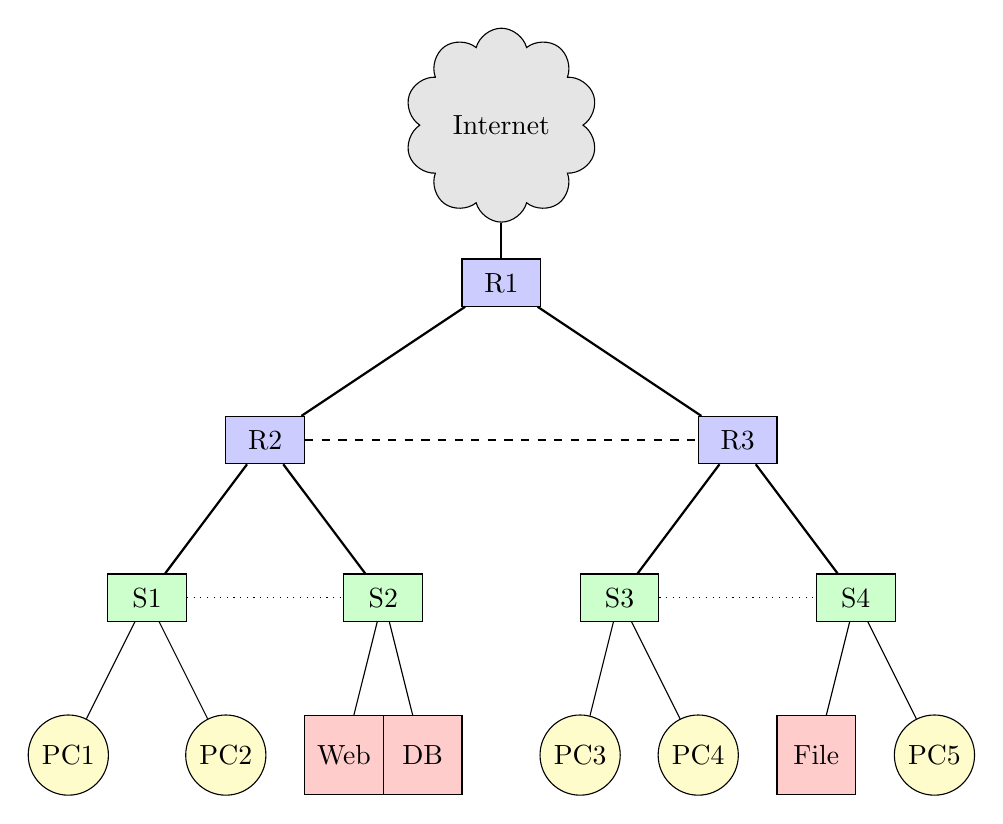
\begin{tikzpicture}[
            node distance=2cm,
            router/.style={rectangle, draw, fill=blue!20, minimum width=1cm, minimum height=0.6cm},
            switch/.style={rectangle, draw, fill=green!20, minimum width=1cm, minimum height=0.6cm},
            computer/.style={circle, draw, fill=yellow!20, minimum size=0.8cm},
            server/.style={rectangle, draw, fill=red!20, minimum width=1cm, minimum height=1cm},
            internet/.style={cloud, draw, fill=gray!20, minimum width=2cm, minimum height=1cm}
        ]

        % Internet cloud
        \node[internet] (internet) at (0,4) {Internet};

        % Core router
        \node[router] (core) at (0,2) {R1};

        % Distribution layer
        \node[router] (r2) at (-3,0) {R2};
        \node[router] (r3) at (3,0) {R3};

        % Access layer switches
        \node[switch] (s1) at (-4.5,-2) {S1};
        \node[switch] (s2) at (-1.5,-2) {S2};
        \node[switch] (s3) at (1.5,-2) {S3};
        \node[switch] (s4) at (4.5,-2) {S4};

        % End devices
        \node[computer] (pc1) at (-5.5,-4) {PC1};
        \node[computer] (pc2) at (-3.5,-4) {PC2};
        \node[server] (srv1) at (-2,-4) {Web};
        \node[server] (srv2) at (-1,-4) {DB};
        \node[computer] (pc3) at (1,-4) {PC3};
        \node[computer] (pc4) at (2.5,-4) {PC4};
        \node[server] (srv3) at (4,-4) {File};
        \node[computer] (pc5) at (5.5,-4) {PC5};

        % Connections
        % Internet to core
        \draw[thick] (internet) -- (core);

        % Core to distribution
        \draw[thick] (core) -- (r2);
        \draw[thick] (core) -- (r3);

        % Distribution to access
        \draw[thick] (r2) -- (s1);
        \draw[thick] (r2) -- (s2);
        \draw[thick] (r3) -- (s3);
        \draw[thick] (r3) -- (s4);

        % Redundant connections between distribution routers
        \draw[thick, dashed] (r2) -- (r3);

        % Access to end devices
        \draw (s1) -- (pc1);
        \draw (s1) -- (pc2);
        \draw (s2) -- (srv1);
        \draw (s2) -- (srv2);
        \draw (s3) -- (pc3);
        \draw (s3) -- (pc4);
        \draw (s4) -- (srv3);
        \draw (s4) -- (pc5);

        % Some cross-connections for redundancy
        \draw[dotted] (s1) -- (s2);
        \draw[dotted] (s3) -- (s4);

    \end{tikzpicture}
    \caption{Computer Network}
    \label{fig:computer-network}
\end{figure}

A computer network enables communication between users and their devices.

\begin{figure}[htbp]
    \centering
    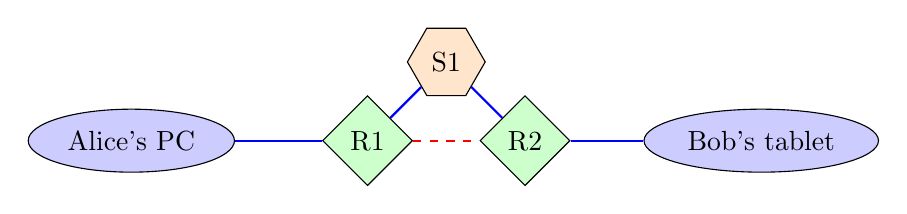
\begin{tikzpicture}[
            node distance=2.5cm,
            user/.style={ellipse, draw, fill=blue!20, minimum width=1.5cm, minimum height=0.8cm},
            device/.style={rectangle, draw, fill=yellow!20, minimum width=1cm, minimum height=0.6cm},
            router/.style={diamond, draw, fill=green!20, minimum width=1cm, minimum height=1cm},
            switch/.style={regular polygon, regular polygon sides=6, draw, fill=orange!20, minimum size=0.8cm}
        ]

        \node[user] (alice) at (-4,0) {Alice's PC};

        \node[user] (bob) at (4,0) {Bob's tablet};

        % Intermediate nodes
        \node[router] (r1) at (-1,0) {R1};
        \node[switch] (s1) at (0,1) {S1};
        \node[router] (r2) at (1,0) {R2};

        % Network path between Alice and Bob
        \draw[thick, blue] (alice) -- (r1);
        \draw[thick, blue] (r1) -- (s1);
        \draw[thick, blue] (s1) -- (r2);
        \draw[thick, blue] (r2) -- (bob);

        % Alternative path (dashed)
        \draw[thick, dashed, red] (r1) -- (r2);

    \end{tikzpicture}
    \caption{Simple Network}
    \label{fig:simple-network}
\end{figure}

The first stop that most home devices take in connecting to other
devices is the router. From there, the router can route data and
find a path for Alice's PC to get to Bob's tablet. The core of any
network is routers, which figure out the best way to get data from
one device to another device.

This process can get complex, with cell tower connections, different ISPs,
different edge devices, and more. Let's abstract the important elements
of the network.

\begin{itemize}
    \item Links: carry data from one endpoint to another
    \item End hosts: sitting at the edge of a network. Generate and receive data.
    \item Routers: forward data through the network.
\end{itemize}

Any network can be abstracted as a connection of links, end hosts, and routers.
We can thus represent any computer network as a graph, in the mathematical
sense, and apply all our graph algorithms to it.

A communication link can either be \emph{full} or \emph{half} duplex.
In a half duplex, a link can carry data in only one direction at a time.
In a full duplex, data transmission is bidirectional.
\marginnote{In this class, all links are assumed to be full duplex
    unless otherwise stated. }
If a link bandwidth is $B$, then a full-duplex link can carry $B$
in both directions simultaneously.
\section{Routing and Packets}

In our abstraction of routers, we leave the problem of finding
a path from end hosts unanswered. Since we can represent a computer
network as a graph, a shortest-path algorithm like Dijkstra's is a
relatively simple way to find a good path between Alice and Bob.
\section{Internet Architecture}

We need to solve these problems:
\begin{itemize}
    \item Name and addressing: identifiers for network nodes
    \item Destination discovery: finding the destination address
    \item Forwarding: sending received data to the next hop (neighbor)
    \item Routing: finding the path from source to destination
    \item Reliability: handling failures, packet drops, packet corruption
    \item Application multiplexing: delivering data from multiple host
          applications to the network and vice versa
\end{itemize}

\subsection{Name and Addressing}
Name is the human-readable name for each node (e.g., URL www.google.com).
Address is where node is located (e.g., IP address 172.21.4.110).

\subsection{Destination discovery}
When you go to a web page, you type the name in your browser. You
need to get the address still. The way names are resolved into
addresses is via the Domain Name System (DNS), a set of global
servers that maintain the mappings between host names and addresses.
When you type a URL, the browser contacts a DNS server to get the address.

\subsection{Forwarding}
A router has many ports. Each port in a router acts as both input
and output, i.e., you can both send and receive packets on each port
simultaneously.
When a packet arrives at a router, the router looks at the destination address
in the header. Based on destination address, the router consults the routing
table, determines the right output port, and sends the packet to that port's queue.
For each output port in parallel, when the port is free, the router picks
a packet from the corresponding output queue in some order (e.g. FIFO) and
sends the packet over the output port.

\subsection{Routing}
How do a network of routers collectively find a path between each
source and destination host? The answer is a routing protocol,
a distributed algorithm that runs independently at each router.


\end{document}